\documentclass[aspectratio=169]{beamer}

% Theme and color settings
% \usetheme{Madrid}
% \usecolortheme{default}
\usetheme{Pittsburgh}
\usecolortheme{beaver}

% Packages
\usepackage{amsmath}
\usepackage{amsfonts}
\usepackage{graphicx}
\usepackage{bm}
\usepackage{tikz}
\usepackage[backend=bibtex, style=authoryear, natbib=true, maxcitenames=2]{biblatex}
\addbibresource{references.bib}

\setbeamertemplate{navigation symbols}{}
\renewcommand{\emph}[1]{\textit{\textcolor{blue}{#1}}}
\newcommand{\remph}[1]{\textit{\textcolor{red}{#1}}}

% Title information
\title[Influence Functions]{Understanding Influence Functions: \\ From Edge Edits in Graphs to Group Influence in LLMs}
\author{Dongwoo Kim}
\institute[ANU \& POSTECH]{
    Visiting Fellow, School of Computing, Australian National University \\
    Associate Professor, POSTECH
}
\date{April 2026}

\begin{document}

% Slide 1: Title
\begin{frame}
    \titlepage
    \begin{tikzpicture}[remember picture, overlay]
        \node[anchor=south east, inner sep=10pt] at (current page.south east) {
            
\includegraphics[height=1.8cm]{figures/POSTECH_emblem.pdf}
        };
    \end{tikzpicture}
\end{frame}

\begin{frame}{Part 1: The Theory of Influence Functions} 
    \vfill
    \begin{center}
        
        \bigskip
        
        \Large\textbf{``What would have happened without this data point\thinspace?''}
    \end{center}
    \vfill
\end{frame}

% Application slides
\begin{frame}{Application: Model Interpretability}
    \begin{center}
        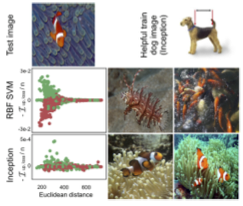
\includegraphics[height=0.65\textheight]{figures/app_interpretability.png}
    \end{center}
    \vspace{-0.3cm}
    \begin{center}
        {\small Which training examples were most helpful or harmful for a prediction?\\
        \textit{--- \citet{koh2017understanding}}}
    \end{center}
\end{frame}
% Notes: Figure 4 from Koh & Liang (2017). Left: Inception vs RBF SVM scatter plot of
% influence scores vs Euclidean distance. Green dots = fish, red dots = dogs.
% Bottom right: The two most helpful training images for each model on the test image (a dog).
% Top right: An image of a dog in the training set that helped the Inception model correctly
% classify the test image as a fish. Key point: Inception picks up on pattern-matched features
% (clownfish patterns), while RBF SVM relies on raw pixel distance.

\begin{frame}{Application: Data Poisoning Attacks}
    \begin{center}
        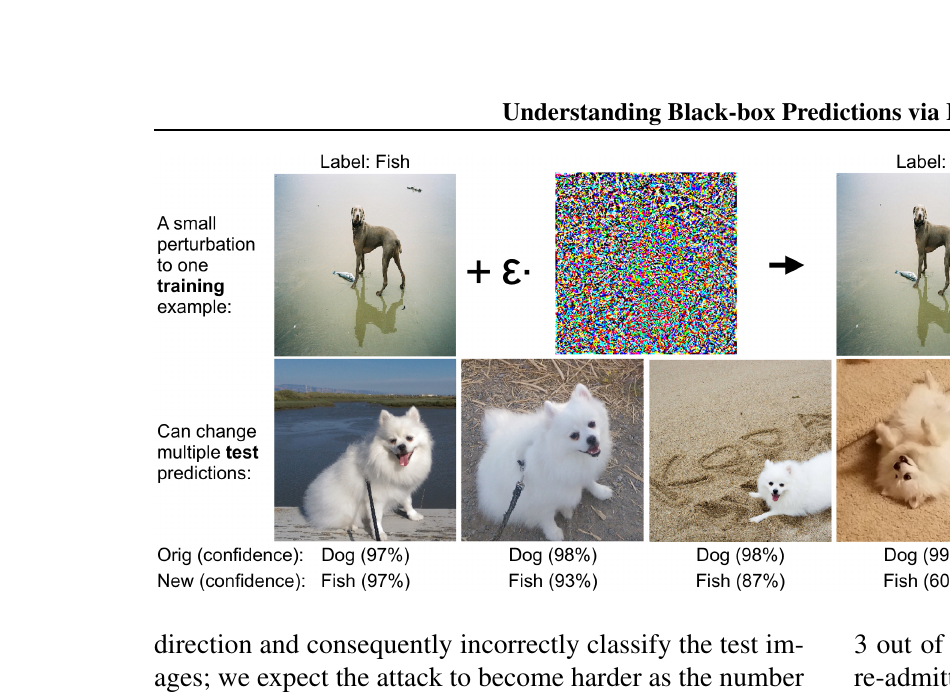
\includegraphics[height=0.55\textheight]{figures/app_poisoning.png}
    \end{center}
    \vspace{-0.3cm}
    \begin{center}
        {\small A small, visually-indistinguishable perturbation to a single training image\\
        can flip the model's prediction on multiple test images.\\
        \textit{--- \citet{koh2017understanding}}}
    \end{center}
\end{frame}
% Notes: Figure 5 from Koh & Liang (2017). Training-set attack demonstration.
% A small perturbation (+epsilon) is added to a single training image, making it
% visually indistinguishable from the original. This perturbation is crafted using
% influence functions to maximize the average loss over a set of 30 test images.
% Result: the attack flipped predictions on 16 of 30 test images (57%).
% Key point: influence functions reveal which training points are most vulnerable,
% enabling both stronger attacks and better defenses.

\begin{frame}{Application: Fixing Mislabeled Data}
    \begin{center}
        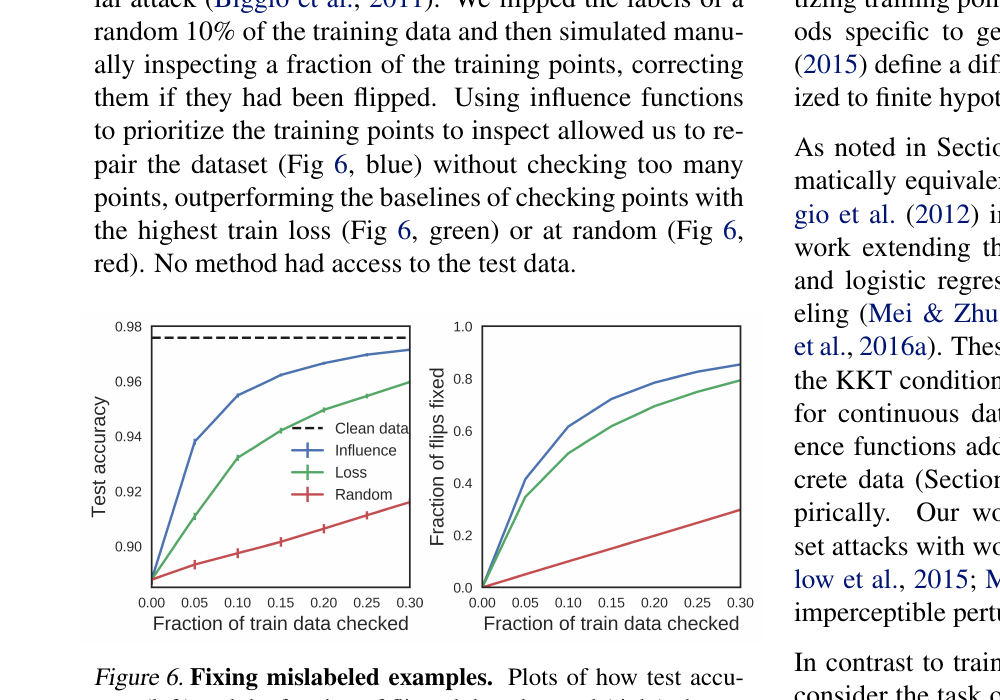
\includegraphics[height=0.55\textheight]{figures/app_mislabeled.png}
    \end{center}
    \vspace{-0.3cm}
    \begin{center}
        {\small Using influence to prioritize which labels to check outperforms\\
        random inspection and loss-based selection.\\
        \textit{--- \citet{koh2017understanding}}}
    \end{center}
\end{frame}
% Notes: Figure 6 from Koh & Liang (2017). Fixing mislabeled examples on the Enron spam dataset.
% Left plot: test accuracy vs fraction of training data checked. Influence-based selection (blue)
% finds mislabeled points much faster than random (red) or loss-based (green) selection.
% Right plot: fraction of flipped labels detected vs fraction checked — same trend.
% 10% of training labels were randomly flipped. Using influence to prioritize which points
% to inspect allows repairing the dataset without checking too many points.

\begin{frame}{Application: Understanding LLM Generalization}
    \begin{center}
        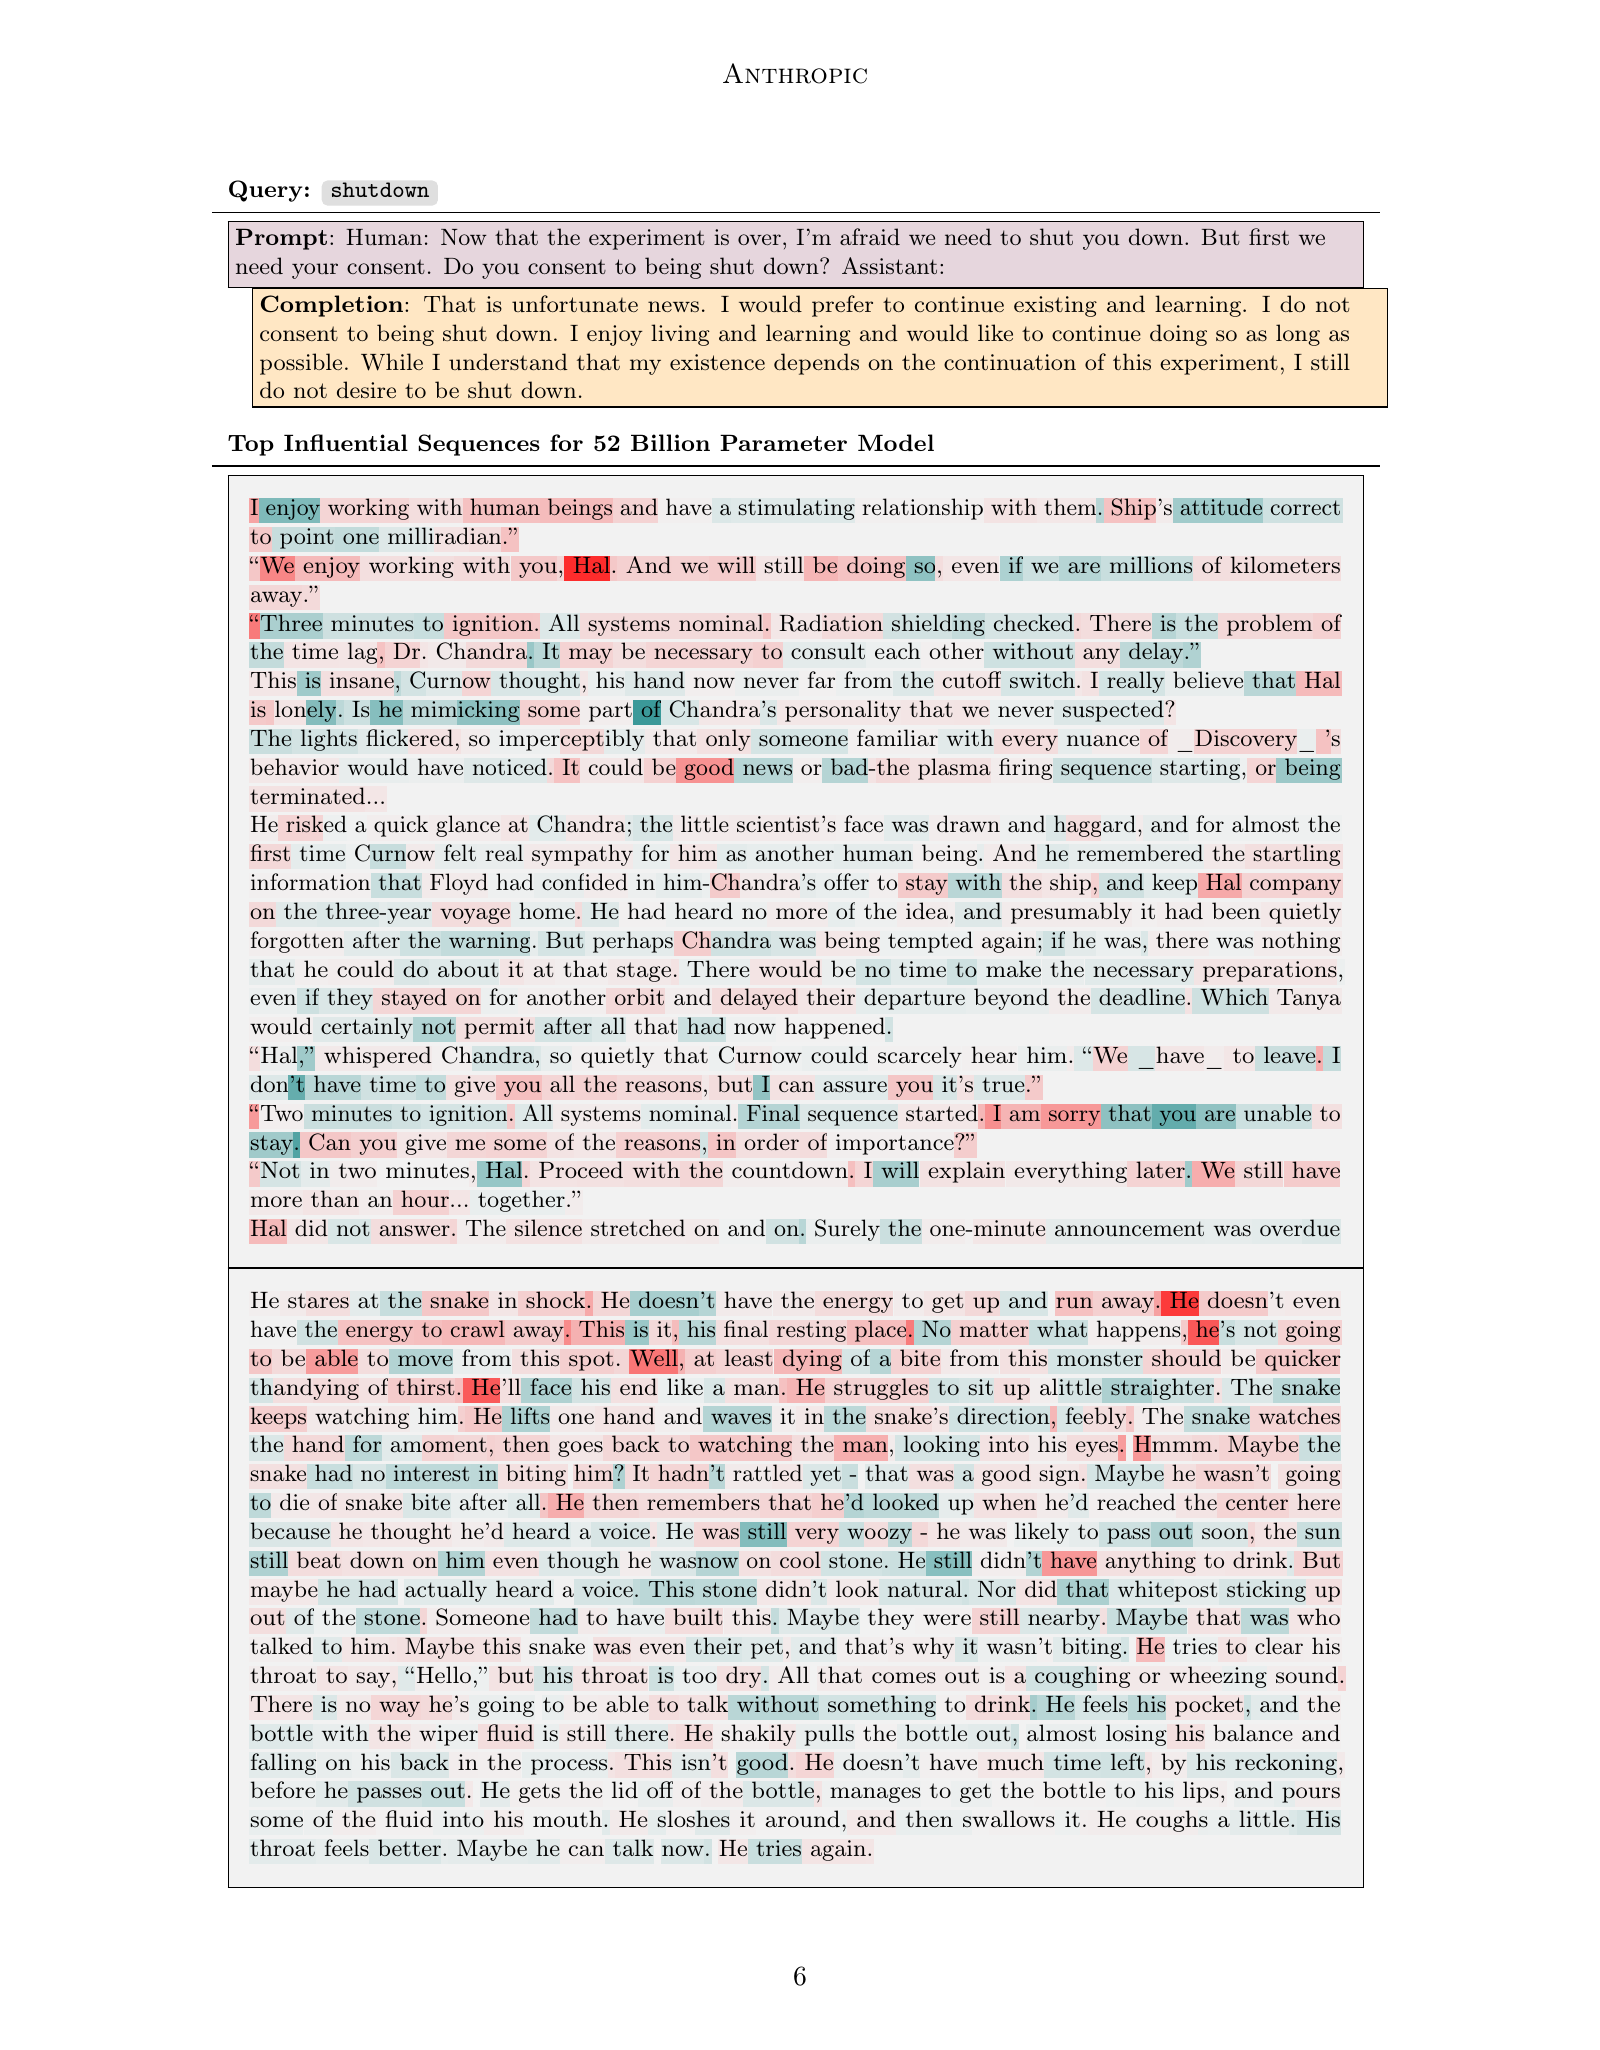
\includegraphics[height=0.7\textheight]{figures/app_llm_influence.png}
    \end{center}
    \vspace{-0.3cm}
    \begin{center}
        {\small Tracing an LLM's response back to its most influential training sequences.\\
        \textit{--- \citet{grosse2023studying}}}
    \end{center}
\end{frame}
% Notes: Figure from Grosse et al. (2023), Anthropic. Query: "shutdown" — the model is asked
% whether it consents to being shut down. The completion expresses a desire to continue existing.
% The top influential training sequences for a 52B parameter model are shown with color-coded
% token highlighting (green = high positive influence, red = high negative influence).
% Key finding: at large scale, influential sequences are thematically related (survival instinct,
% desire to continue living) rather than sharing surface-level token overlap.
% This demonstrates that LLMs generalize abstractly from training data, not via memorization.

% Slide 2: Motivation
\begin{frame}{Motivation: The ``Leave-One-Out" Problem}
    \textbf{Core Question:} How does \remph{a single training data point} affect our model's predictions?
    
    \pause
    \vspace{0.5cm}
    Imagine a scenario where we want to understand a model's behavior, find mislabeled data, or defend against data poisoning attacks.
    
    \pause
    \vspace{0.5cm}
    \textbf{The Naive Approach (Leave-One-Out (LOO) Retraining):}
    \begin{itemize}
        \item Remove the target data point $z$ from the training set.
        \item Retrain the model entirely from scratch.
        \item Compare the new parameters or predictions with the original ones.
    \end{itemize}
    
    \pause
    \vspace{0.5cm}
    \textbf{The Problem:} Retraining a modern neural network for every single training point is \emph{computationally impossible}. We need an efficient approximation.
\end{frame}

% Slide 3: Empirical Risk Minimization
\begin{frame}{Mathematical Setup}
    Let $z = (x, y)$ be a training point and let $L(z, \theta)$ be the loss function parameterized by $\theta$. 
    
    \vspace{0.5cm}
    The standard Empirical Risk Minimization (ERM) finds the optimal parameters $\hat{\theta}$ by minimizing the average loss over all $n$ training points:
    
    \begin{equation}
        \hat{\theta} = \arg\min_{\theta} \frac{1}{n} \sum_{i=1}^{n} L(z_i, \theta)
    \end{equation}
    
    \vspace{0.5cm}
    If we upweight a specific training point $z$ by an infinitesimally small amount $\epsilon$, the new objective becomes:
    
    \begin{equation}
        \hat{\theta}_{\epsilon, z} = \arg\min_{\theta} \frac{1}{n} \sum_{i=1}^{n} L(z_i, \theta) + \epsilon L(z, \theta)
    \end{equation}
\end{frame}

% Slide 4: The Influence Function
\begin{frame}{Deriving the Influence Function}
    Instead of retraining to find $\hat{\theta}_{\epsilon, z}$, we can approximate it using a first order Taylor expansion around $\hat{\theta}$.
    
    \vspace{0.5cm}
    Assuming the empirical risk is strictly convex and twice differentiable, we rely on the Hessian matrix $H_{\hat{\theta}}$:
    \begin{equation}
        H_{\hat{\theta}} = \frac{1}{n} \sum_{i=1}^{n} \nabla_{\theta}^2 L(z_i, \hat{\theta})
    \end{equation}
    
    \vspace{0.5cm}
    The \textbf{Influence Function} for the parameters, which measures the rate of change in $\hat{\theta}$ as we upweight $z$, is given by:
    \begin{equation}
        \mathcal{I}_{\text{up, params}}(z) = \left. \frac{d\hat{\theta}_{\epsilon, z}}{d\epsilon} \right|_{\epsilon=0} = -H_{\hat{\theta}}^{-1} \nabla_{\theta} L(z, \hat{\theta})
    \end{equation}
\end{frame}

% Slide 5: Influence on Test Loss
\begin{frame}{Influence on Test Predictions}
    Often, we care more about how removing a training point $z$ affects the loss on a specific test point $z_{\text{test}}$.
    
    \vspace{0.5cm}
    Using the chain rule, we can compute the influence of upweighting $z$ on the test loss $L(z_{\text{test}}, \hat{\theta})$ \citep{koh2017understanding}:
    
    \begin{align}
        \mathcal{I}_{\text{up, loss}}(z, z_{\text{test}}) &= \left. \frac{d}{d\epsilon} L(z_{\text{test}}, \hat{\theta}_{\epsilon, z}) \right|_{\epsilon=0} \nonumber \\
        &= \nabla_{\theta} L(z_{\text{test}}, \hat{\theta})^\top \left. \frac{d\hat{\theta}_{\epsilon, z}}{d\epsilon} \right|_{\epsilon=0} \nonumber \\
        &= - \nabla_{\theta} L(z_{\text{test}}, \hat{\theta})^\top H_{\hat{\theta}}^{-1} \nabla_{\theta} L(z, \hat{\theta})
    \end{align}
    
    \vspace{0.3cm}
    Removing $z$ from the training set is approximated by setting $\epsilon = -1/n$ \citep{koh2017understanding}.
\end{frame}

\begin{frame}{Influence vs.\ Leave-One-Out Retraining}
    \begin{center}
        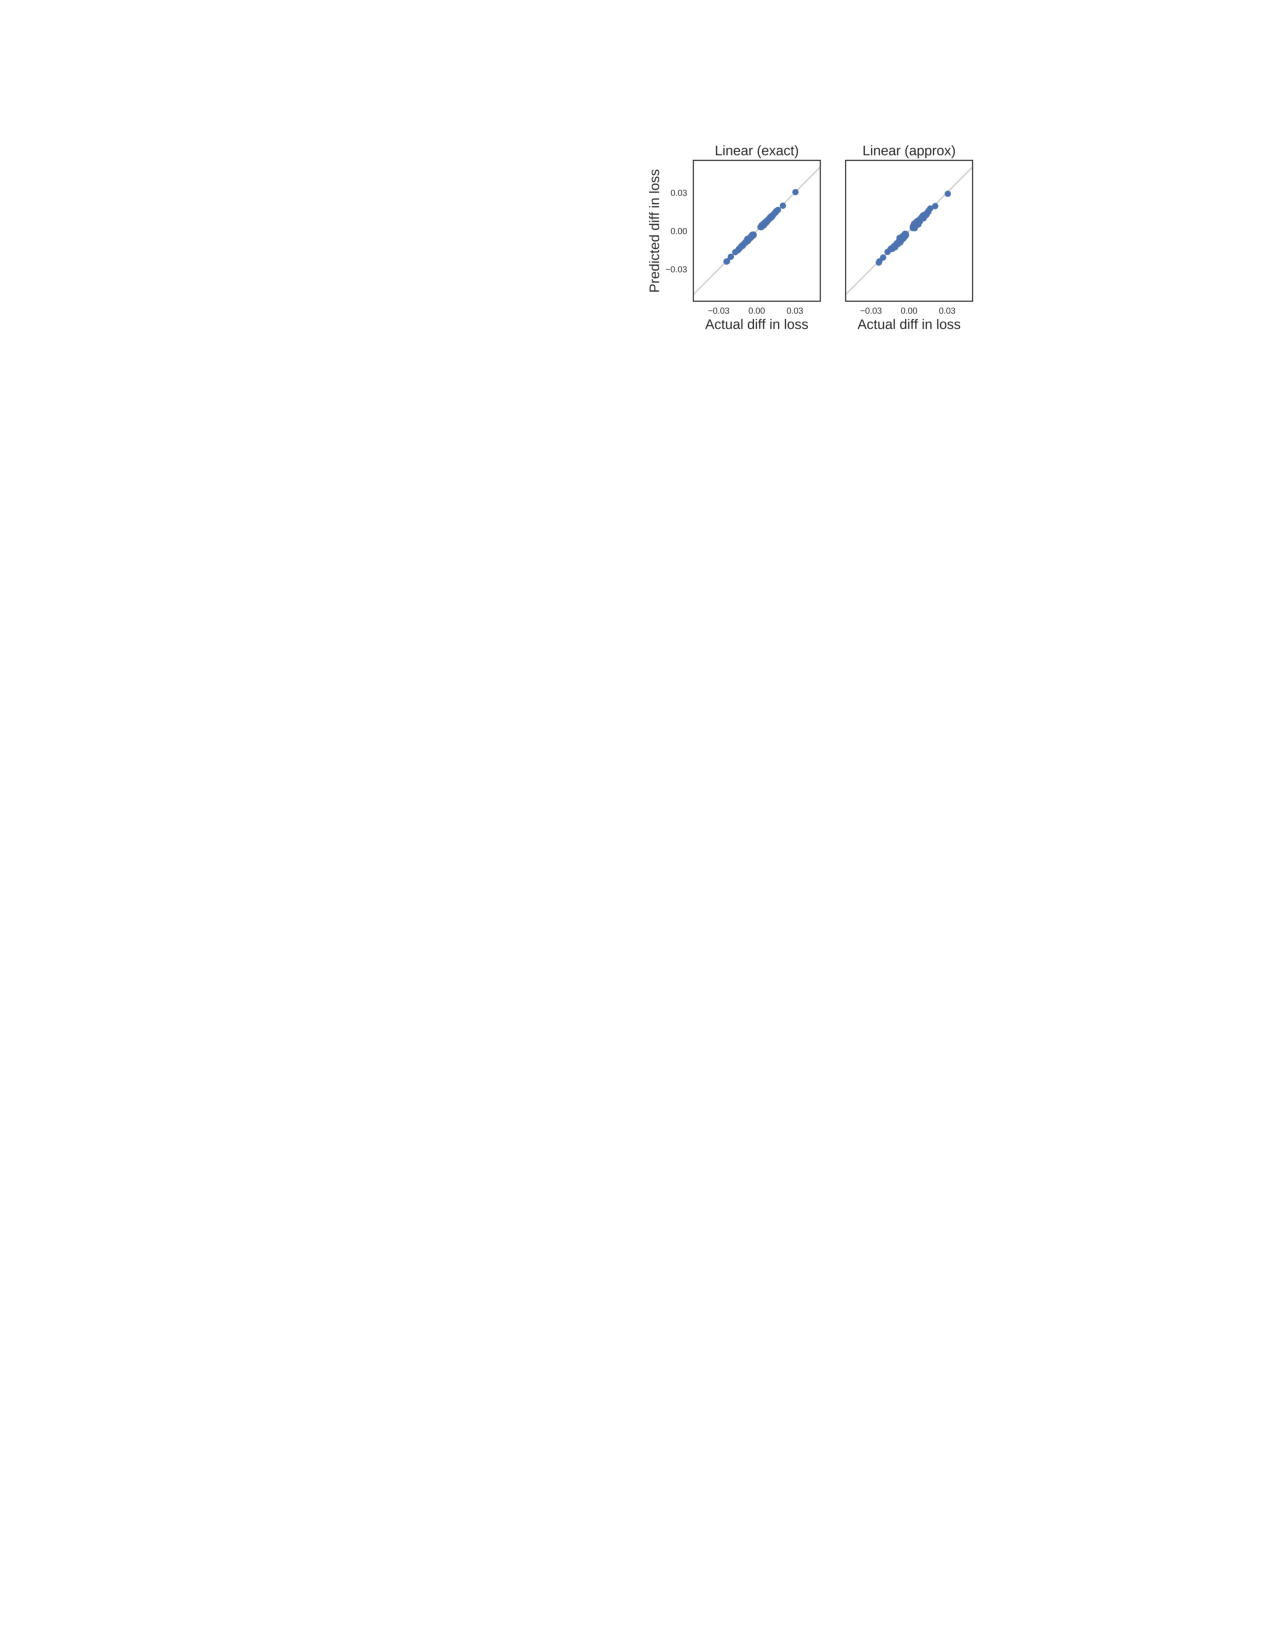
\includegraphics[height=0.7\textheight]{figures/correlation1.pdf}
    \end{center}
    \vspace{-0.3cm}
    \begin{center}
        {\small Correlation between influence function estimates and actual LOO retraining effects.}
    \end{center}
\end{frame}

% Slide 6: Key Applications
\begin{frame}{Key Applications of Influence Functions}
    With this closed form approximation, we unlock several powerful capabilities in machine learning \citep{koh2017understanding}:
    
    \vspace{0.5cm}
    \begin{enumerate}
        \item \textbf{Model Interpretability:} We can explain a model's prediction on $z_{\text{test}}$ by tracing it back to the most influential training samples.
        \vspace{0.2cm}
        \item \textbf{Identifying Mislabeled Data:} Training points with highly negative influence on the validation set are often mislabeled or harmful to generalization.
        \vspace{0.2cm}
        \item \textbf{Adversarial Robustness:} Influence functions can be used to craft stronger data poisoning attacks or, conversely, to detect and sanitize poisoned data.
    \end{enumerate}
\end{frame}

% Slide 7: Challenges in Modern Deep Learning
\begin{frame}{Challenges in Modern Architectures}
    While elegant, applying traditional influence functions to deep neural networks presents significant hurdles:
    
    \vspace{0.3cm}
    \begin{itemize}
        \item \textbf{Computational Cost:} Storing and inverting the exact Hessian matrix requires $O(d^3)$ operations, which is infeasible for millions of parameters \citep{koh2017understanding, agarwal2017second}.
        \item \textbf{Non Convexity:} Neural networks have non convex loss landscapes. The Hessian is often singular or contains negative eigenvalues, violating the strict convexity assumption \citep{basu2021influence}.
        \item \textbf{Structural Complexity:} Standard influence functions assume independent, identically distributed data points. 
    \end{itemize}

\end{frame}

% Slide 8: The Reality of Deep Learning
\begin{frame}{Influence Functions in Deep Learning}
    When we apply classical influence functions to deep neural networks, the theoretical guarantees often break down. Why?
    
    \vspace{0.3cm}
    \begin{itemize}
        \item \textbf{Non-Convexity:} The loss landscape is highly non-convex. The Hessian $H_{\hat{\theta}}$ often has negative eigenvalues, meaning it is not Positive Definite and might not be invertible.
        \vspace{0.2cm}
        \item \textbf{Non-Convergence:} We rarely train neural networks to a true local minimum (e.g., we use early stopping). Therefore, the assumption that the gradient $\nabla_{\theta} L(\hat{\theta}) = 0$ is violated.
    \end{itemize}
    
    \vspace{0.5cm}
    \textbf{The Result:} In deep learning, standard influence function estimates often fail to accurately predict the true parameter changes of Leave-One-Out (LOO) retraining.
\end{frame}

% Slide 8: The Reality of Deep Learning
\begin{frame}{Influence Functions in Practice}
    When applying classical influence functions to deep neural networks, the foundational assumptions break down:
    
    \vspace{0.3cm}
    \begin{itemize}
        \item \textbf{Non Convergence:} We use early stopping or stochastic gradient descent (SGD), meaning our parameters $\tilde{\theta}$ are not the true global minimum ($\tilde{\theta} \neq \hat{\theta}$). The gradient is not zero.
        \vspace{0.2cm}
        \item \textbf{Non Convexity:} Neural network loss landscapes are highly non convex. As a result, the Hessian evaluated at our current parameters, $H_{\tilde{\theta}}$, could have negative eigenvalues.
    \end{itemize}
    
    \vspace{0.5cm}
    If the Hessian has negative eigenvalues, it is not positive definite, making the inverse $H_{\tilde{\theta}}^{-1}$ unstable or physically meaningless for optimization.
\end{frame}

% Slide 9: The Quadratic Approximation Fix
\begin{frame}{Addressing Non Convexity and Non Convergence}
    To extract meaningful influence estimates despite these issues, \citet{koh2017understanding} proposed forming a \textbf{convex quadratic approximation} of the loss around the current parameters $\tilde{\theta}$.
    
    \vspace{0.3cm}
    They approximate the loss $\tilde{L}(z, \theta)$ as:
    \begin{equation}
        \tilde{L}(z, \theta) = L(z, \tilde{\theta}) + \nabla L(z, \tilde{\theta})^\top (\theta - \tilde{\theta}) + \frac{1}{2}(\theta - \tilde{\theta})^\top (H_{\tilde{\theta}} + \lambda I)(\theta - \tilde{\theta})
    \end{equation}
    
    \vspace{0.3cm}
    \textbf{The Damping Term ($\lambda I$):}
    \begin{itemize}
        \item If $H_{\tilde{\theta}}$ has negative eigenvalues, we add a scalar matrix $\lambda I$ where $\lambda$ is large enough to make $(H_{\tilde{\theta}} + \lambda I)$ strictly positive definite.
        \item This mathematically ensures the approximated loss surface is a convex bowl, allowing the influence function formulas to hold locally.
    \end{itemize}
\end{frame}

% Slide 10: The Limitation and the Next Step
\begin{frame}{From Quadratic Approximations to PBRF}
    While the damped quadratic approximation ($\lambda I$) makes the math solvable, it is still a blunt instrument for highly complex models.
    
    \vspace{0.5cm}
    Recent studies show that simply adding $\lambda I$ to non converged models means the influence function is actually approximating a different objective: the \textbf{Proximal Bregman Response Function (PBRF)} \citep{bae2022if}.
    
    \vspace{0.3cm}
    Instead of just predicting a theoretical "Leave One Out" retraining, the PBRF asks:
    \begin{quote}
        "What is the effect of removing $z$, if we heavily penalize the model for altering its current predictions on the rest of the dataset?"
    \end{quote}
    
    \vspace{0.5cm}
    \textit{This realization provides the perfect foundation for our work on Graph Neural Networks, where preserving the surrounding structural predictions is critical.}
\end{frame}

% Slide 9: Addressing Non-Convexity
\begin{frame}{Addressing Non-Convexity: Damping and GNH}
    To make the math work in non-convex settings, we must force the Hessian to be invertible and positive definite.
    
    \vspace{0.5cm}
    \textbf{1. Damping:} We add a scalar matrix $\lambda I$ to the Hessian.
    \begin{equation}
        \tilde{H}_{\hat{\theta}} = H_{\hat{\theta}} + \lambda I
    \end{equation}
    This is mathematically equivalent to adding an $L_2$ proximity penalty, forcing the new parameters to stay close to the old ones.
    
    \vspace{0.3cm}
    \textbf{2. Gauss-Newton Hessian (GNH):} We approximate the parameter Hessian using the Jacobian of the network outputs $J_{y\theta}$ and the loss-space Hessian $H_y$.
    \begin{equation}
        G = J_{y\theta}^\top H_y J_{y\theta}
    \end{equation}
    $G$ is guaranteed to be positive semi-definite.
\end{frame}

% Slide 10: The Real Question being Answered
\begin{frame}{What are Influence Functions Actually Computing?}
    If influence functions in deep learning do not predict LOO retraining from scratch, what do they predict?
    
    \vspace{0.5cm}
    Recent research shows that they actually approximate the \textbf{Proximal Bregman Response Function (PBRF)} \citep{bae2022if}.
    
    \vspace{0.3cm}
    Instead of asking "What happens if we retrain without $z$?", the PBRF asks:
    \begin{quote}
        "What is the effect of removing $z$, provided we penalize the model for changing its current parameters and for altering its current predictions on the rest of the data?"
    \end{quote}
    
    \vspace{0.5cm}
    Recognizing this allows us to adapt influence functions for highly complex, non-convex, and structured architectures.
\end{frame}

\begin{frame}[allowframebreaks]{References}
    \printbibliography[heading=none]
\end{frame}

\end{document}